\chapter{Design}

This chapter outlines an overview of the design of the project and why certain decisions were made
regarding the design. To help with this, sections on the dataset and research methodology used
have also been included to give a better view of the entire system.

%You should concentrate on the more important aspects of the design. It is essential that an overview is presented before going into detail. As well as describing the design adopted it must also explain what other designs were considered and why they were rejected.

%The design should describe what you expected to do, and might also explain areas that you had to revise after some investigation.

%Typically, for an object-oriented design, the discussion will focus on the choice of objects and classes and the allocation of methods to classes. The use made of reusable components should be described and their source referenced. Particularly important decisions concerning data structures usually affect the architecture of a system and so should be described here.

%How much material you include on detailed design and implementation will depend very much on the nature of the project. It should not be padded out. Think about the significant aspects of your system. For example, describe the design of the user interface if it is a critical aspect of your system, or provide detail about methods and data structures that are not trivial. Do not spend time on long lists of trivial items and repetitive descriptions. If in doubt about what is appropriate, speak to your supervisor.


\section{The Image Dataset}
The image dataset consists of 325 paintings, with associated metadata. Metadata
includes title, year or year ranges (for those works where year is unknown but
can be estimated by curators), genre, original painting size, painting
materials and image size.

These photographs of paintings are challenging themselves: they are
not colour calibrated; some suffer from reflections (towards the end of his
life Kyffin painted using exceptionally thick and textural strokes, which gives
specularities on the catalogue images); they are at varying resolutions; and
come from a range of different cameras. Image size bears little relation to the
original painting size, and some images are even optimised for the web.
Table~\ref{summary_t} below summarises the dataset.

\begin{table}[h]
\centering
\begin{tabular}{| l | c | c | p{3cm} |}
\hline
Type & Number & Number & Notes \\
  & & (Known date) &  \\
\hline
Landscapes  & 247 & 64 & \\
Portraits   &  52 & 35 & \\
Seascapes   &  11 &  2 & \\
Still lifes &   4 &  1 & \\
Other       &   8 &  0 & Other or studies \\
\hline
\end{tabular}
\caption{A summary of the Kyffin Williams painting dataset
\label{summary_t}}
\end{table}

\section{Methodology}

Within the database of 325 paintings, the actual year of painting is known for 102 artworks. 
To judge how well an analysis technique performs a leave-one-out cross validation methodology is
applied to each technique, only working with these 102 artworks so that any amount of uncertainty 
is removed.

Leave-one-out cross validation involves taking a painting for which the year is known, then use
the classifier to guess the year; this allows the result to be validated against the known year,
thereby showing how well a given analysis technique works.

To simplify the classification stage a $k$-Nearest Neighbour classifier is used with the remaining
101 paintings for which the date is known. $k$-Nearest neighbour is a fast, non-parametric classifier.
It has the advantage of being easy to implement and makes no assumptions about the underlying patterns in the data.
Only the other paintings which are similarly located in the feature space are considered as part of this process.
This functions on the assumption that paintings similarly located in feature space are also similarly located in time,
this will be the case if an analysis technique is performing well. Figure \ref{img:classification-overview} shows this process.

\begin{figure}[h]
\centering
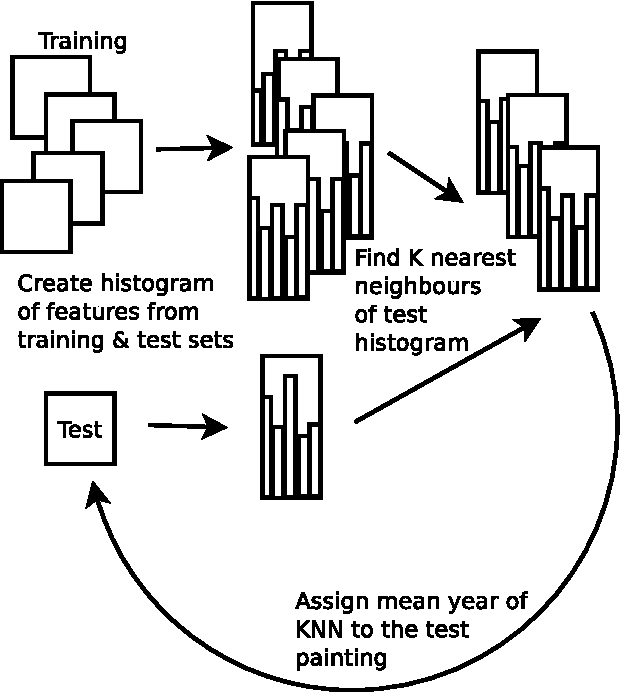
\includegraphics[width=0.4\textwidth]{img/kyffin_overview.pdf}
\caption{Overview of the Classification Methodology}
\label{img:classification-overview}
\end{figure}


\section{Overall Architecture}
The basic architecture for any system like this is to load the data in from a source,
apply an analysis technique to each member of the dataset then pass this data into the classification system. 
The results of this system should return the classified and actual year for each member of the dataset.
These results can then have cross validation performed on them. This architecture is summed up in
Figure~\ref{fig:basic-arch}.

\begin{figure}[h]
\centering
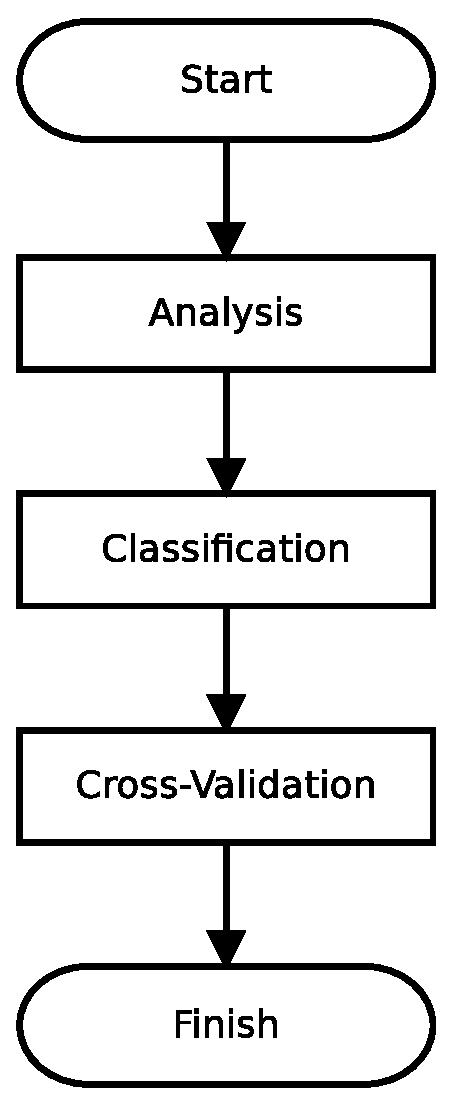
\includegraphics[scale=0.4]{img/basic-arch}
\caption{Basic Overall Architecture}\label{fig:basic-arch}
\end{figure}

Building up from this it is apparent that to implement the analysis and classification steps that 
there is a need to implement the factory method design 
pattern\cite[p.~107-117]{Gamma1996Design}. Reading from a data source should be a simple
matter of reading from a file, and cross validation has already been decided upon: leave-one-out
cross validation.
Figure~\ref{fig:factory-arch} shows the design after adding in the factory methods.

\begin{figure}[h]
\centering
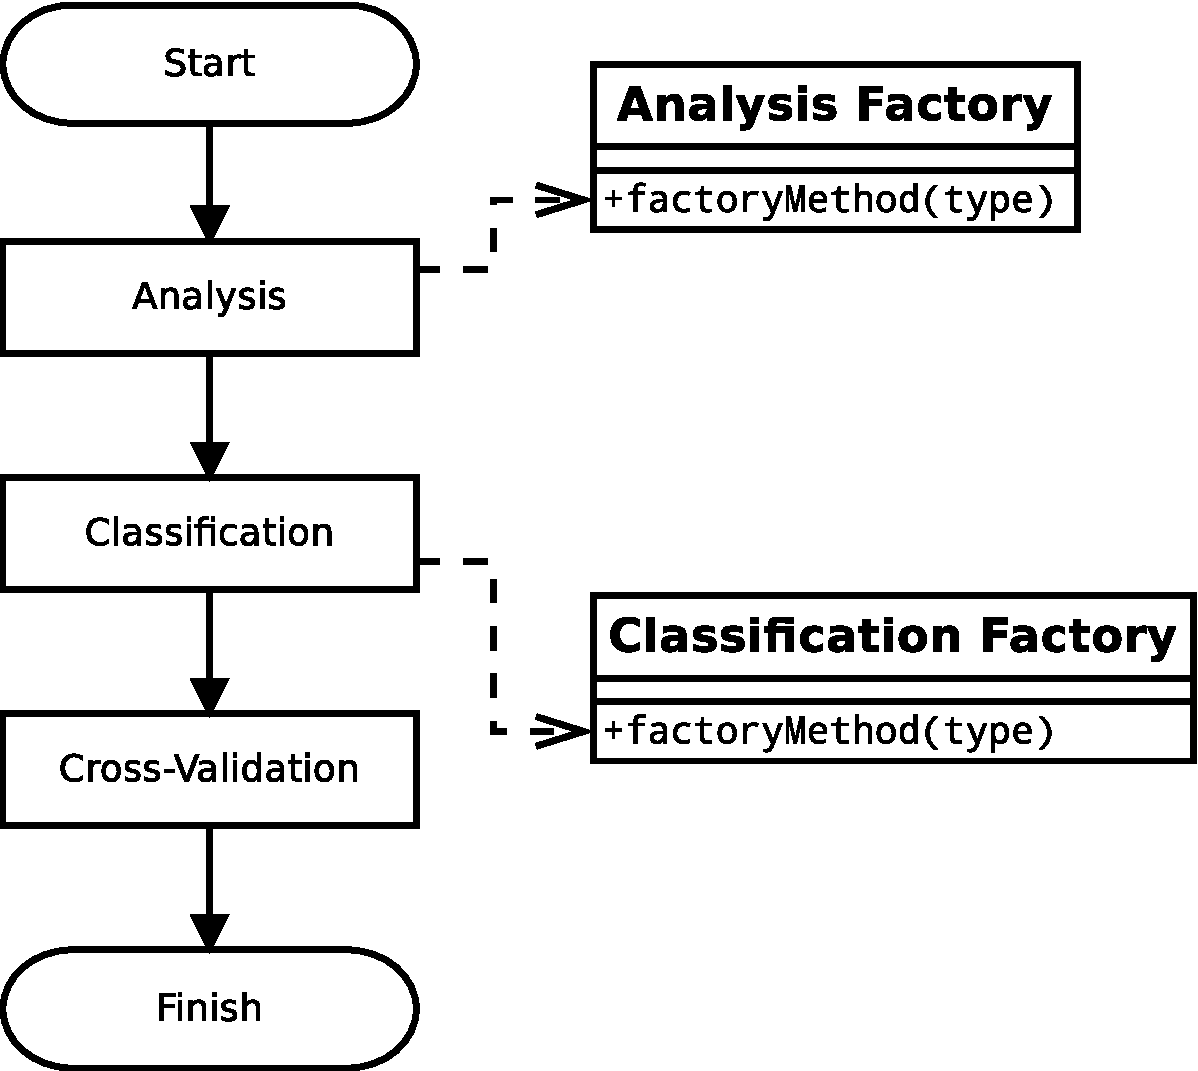
\includegraphics[scale=0.4]{img/factory-arch}
\caption{Overall Architecture with Factory Methods}\label{fig:factory-arch}
\end{figure}

From this there is the need for two top-level interfaces \verb+Analyser+ and \verb+Classifier+. The 
\verb+Analyser+ interface should have a single method which runs analysis on a painting and return
some form of object which represents the analysed data.

The \verb+Classifier+ class should have a method which takes a single painting and a set of
paintings, returning the classified year of the single painting based on the set
of paintings.

At this point it is also required that there is a class to store the metadata of a painting. 
Figure~\ref{fig:interfaces-arch} depicts the design after adding in these parts.

\begin{figure}[h]
\centering
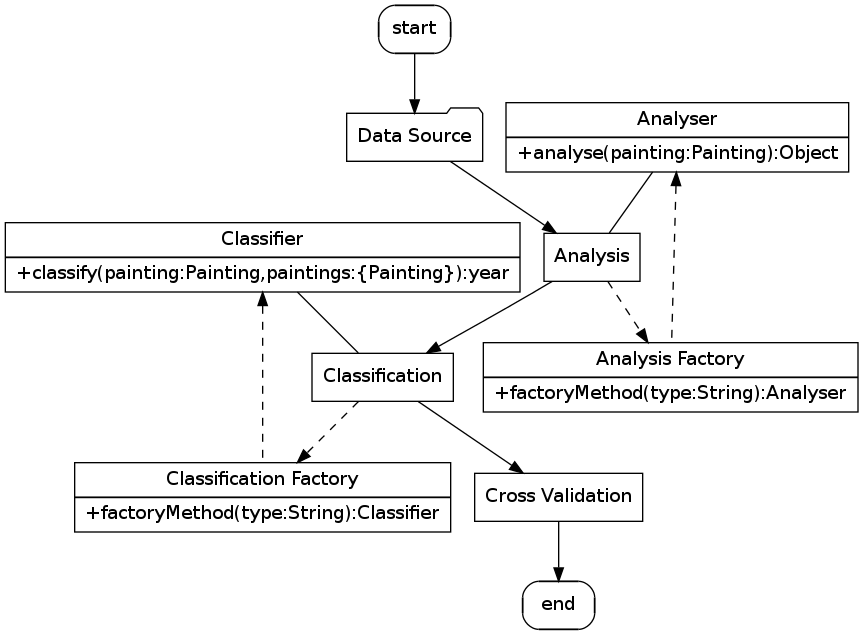
\includegraphics[scale=0.4]{img/interfaces-arch}
\caption{Overall architecture with Interfaces for Analysers and Classifiers}\label{fig:interfaces-arch}
\end{figure}

From this the concrete techniques were implemented, at points it became necessary to add additional 
methods to the interfaces with some abstract implementation. This was particularly
apparent during the change to \gls{cv2} where all results from analysis techniques became 
histograms. The distance method in the \texttt{Analyser} interface was then implemented to call
the \gls{opencv} compare histogram method. This allowed the distance technique to always use 
the same measure of distance, allowing the analysis techniques to be compared more fairly.

With exemplars it was also useful to implement a centroid method as part of the \texttt{Analyser}
interface. This was necessary to ensure the method for determining the centre point was the same. This highlights the 
usefulness of constantly evolving the design using the rapid prototyping methodology.

Until this point the inheritance had been unnecessary due to Python's duck typing. This inheritance had been
purely to help the author understand the architecture. After this point the properties of 
object-orientation were being leveraged to help reduce the amount of repeated code.

\subsection{GUI Elements}

Initially a GUI Factory was implemented to display the results from the techniques graphically, 
using the same sort of method that had been used for the analysis and classification 
techniques. However, as the project continued the focus shifted away from this section due to
the importance of other sections of work. Initially this was a part of the design and was included 
as a part of the progress report; shown in Figure~\ref{fig:prog-design}. This also 
includes details of which methods each interface would include.


\begin{figure}[h!]
\centering
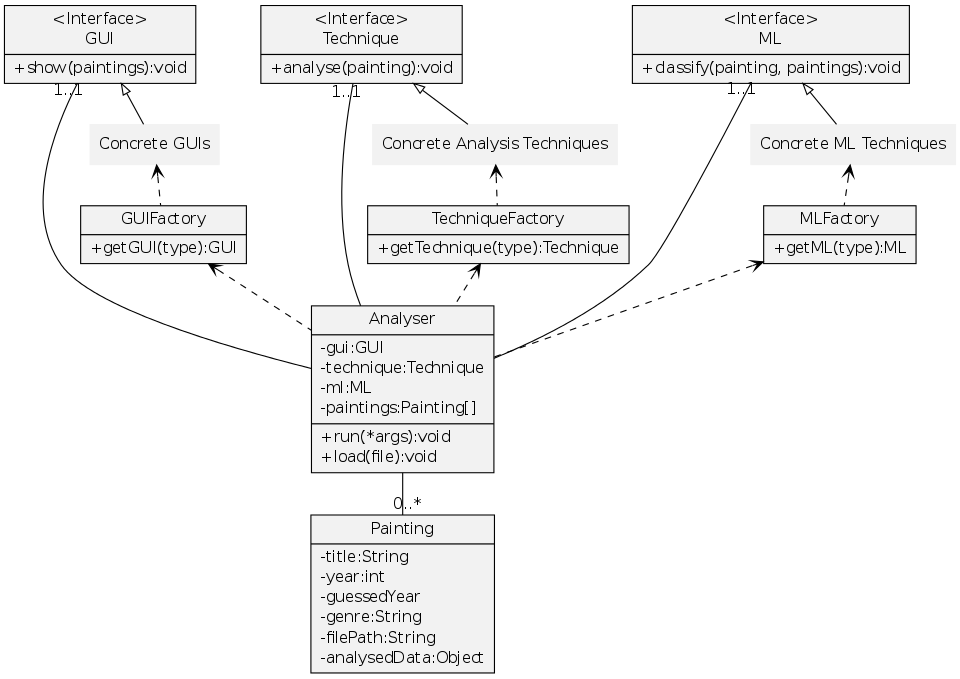
\includegraphics[width=\textwidth]{../ProgressReport/img/design.png}
\caption{Initial Design from the Progress Report}\label{fig:prog-design}
\end{figure}

It should also be noted that of the time of writing the progress report some of the classes had
different names, these were later refactored to better describe the functionality they perform.
Figure~\ref{fig:uml} shows a better version of the class design with these changes in mind and
with the GUI elements removed to keep the design simplistic.

\begin{figure}[h]
\centering
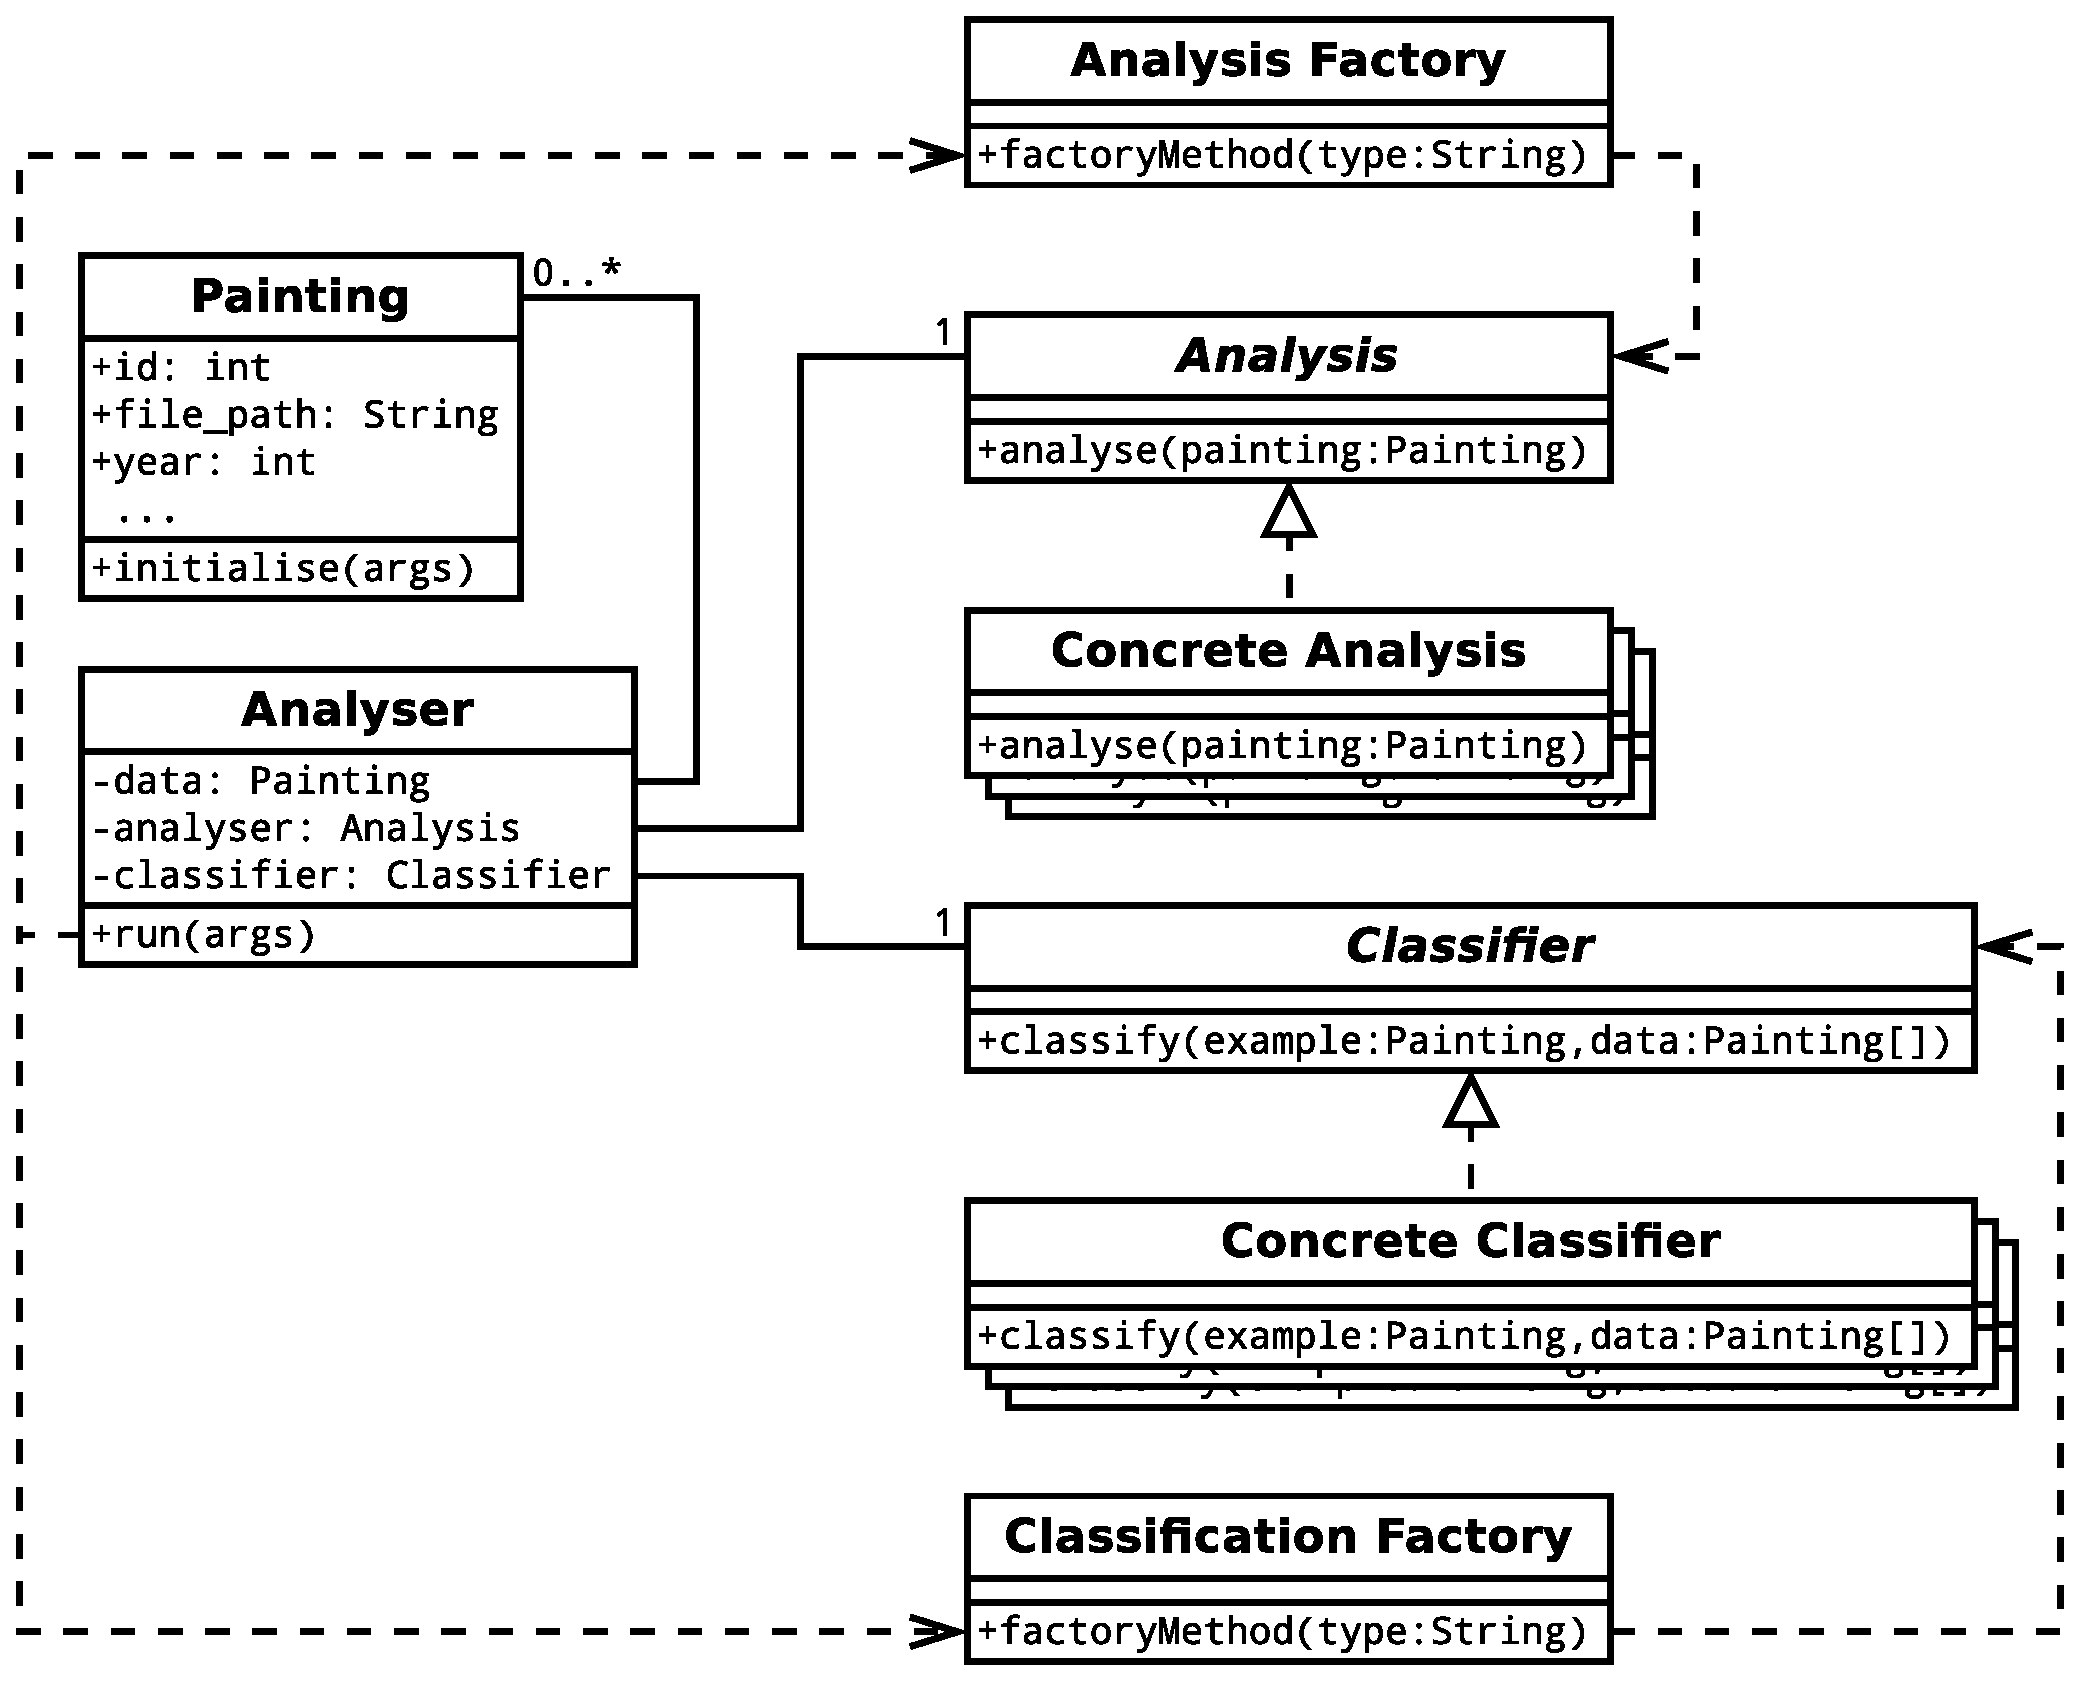
\includegraphics[width=0.75\textwidth]{img/uml}
\caption{Overall class design}\label{fig:uml}
\end{figure}

These methods inevitably changed as the design evolved; mainly to add extra functionality whilst
keeping the re-use of code down, as good object-orientated design should do. The evolutionary 
nature of the methodology allowed for this. Figure~\ref{fig:uml-final} shows the updates to the
class design.

\begin{figure}[h]
\centering
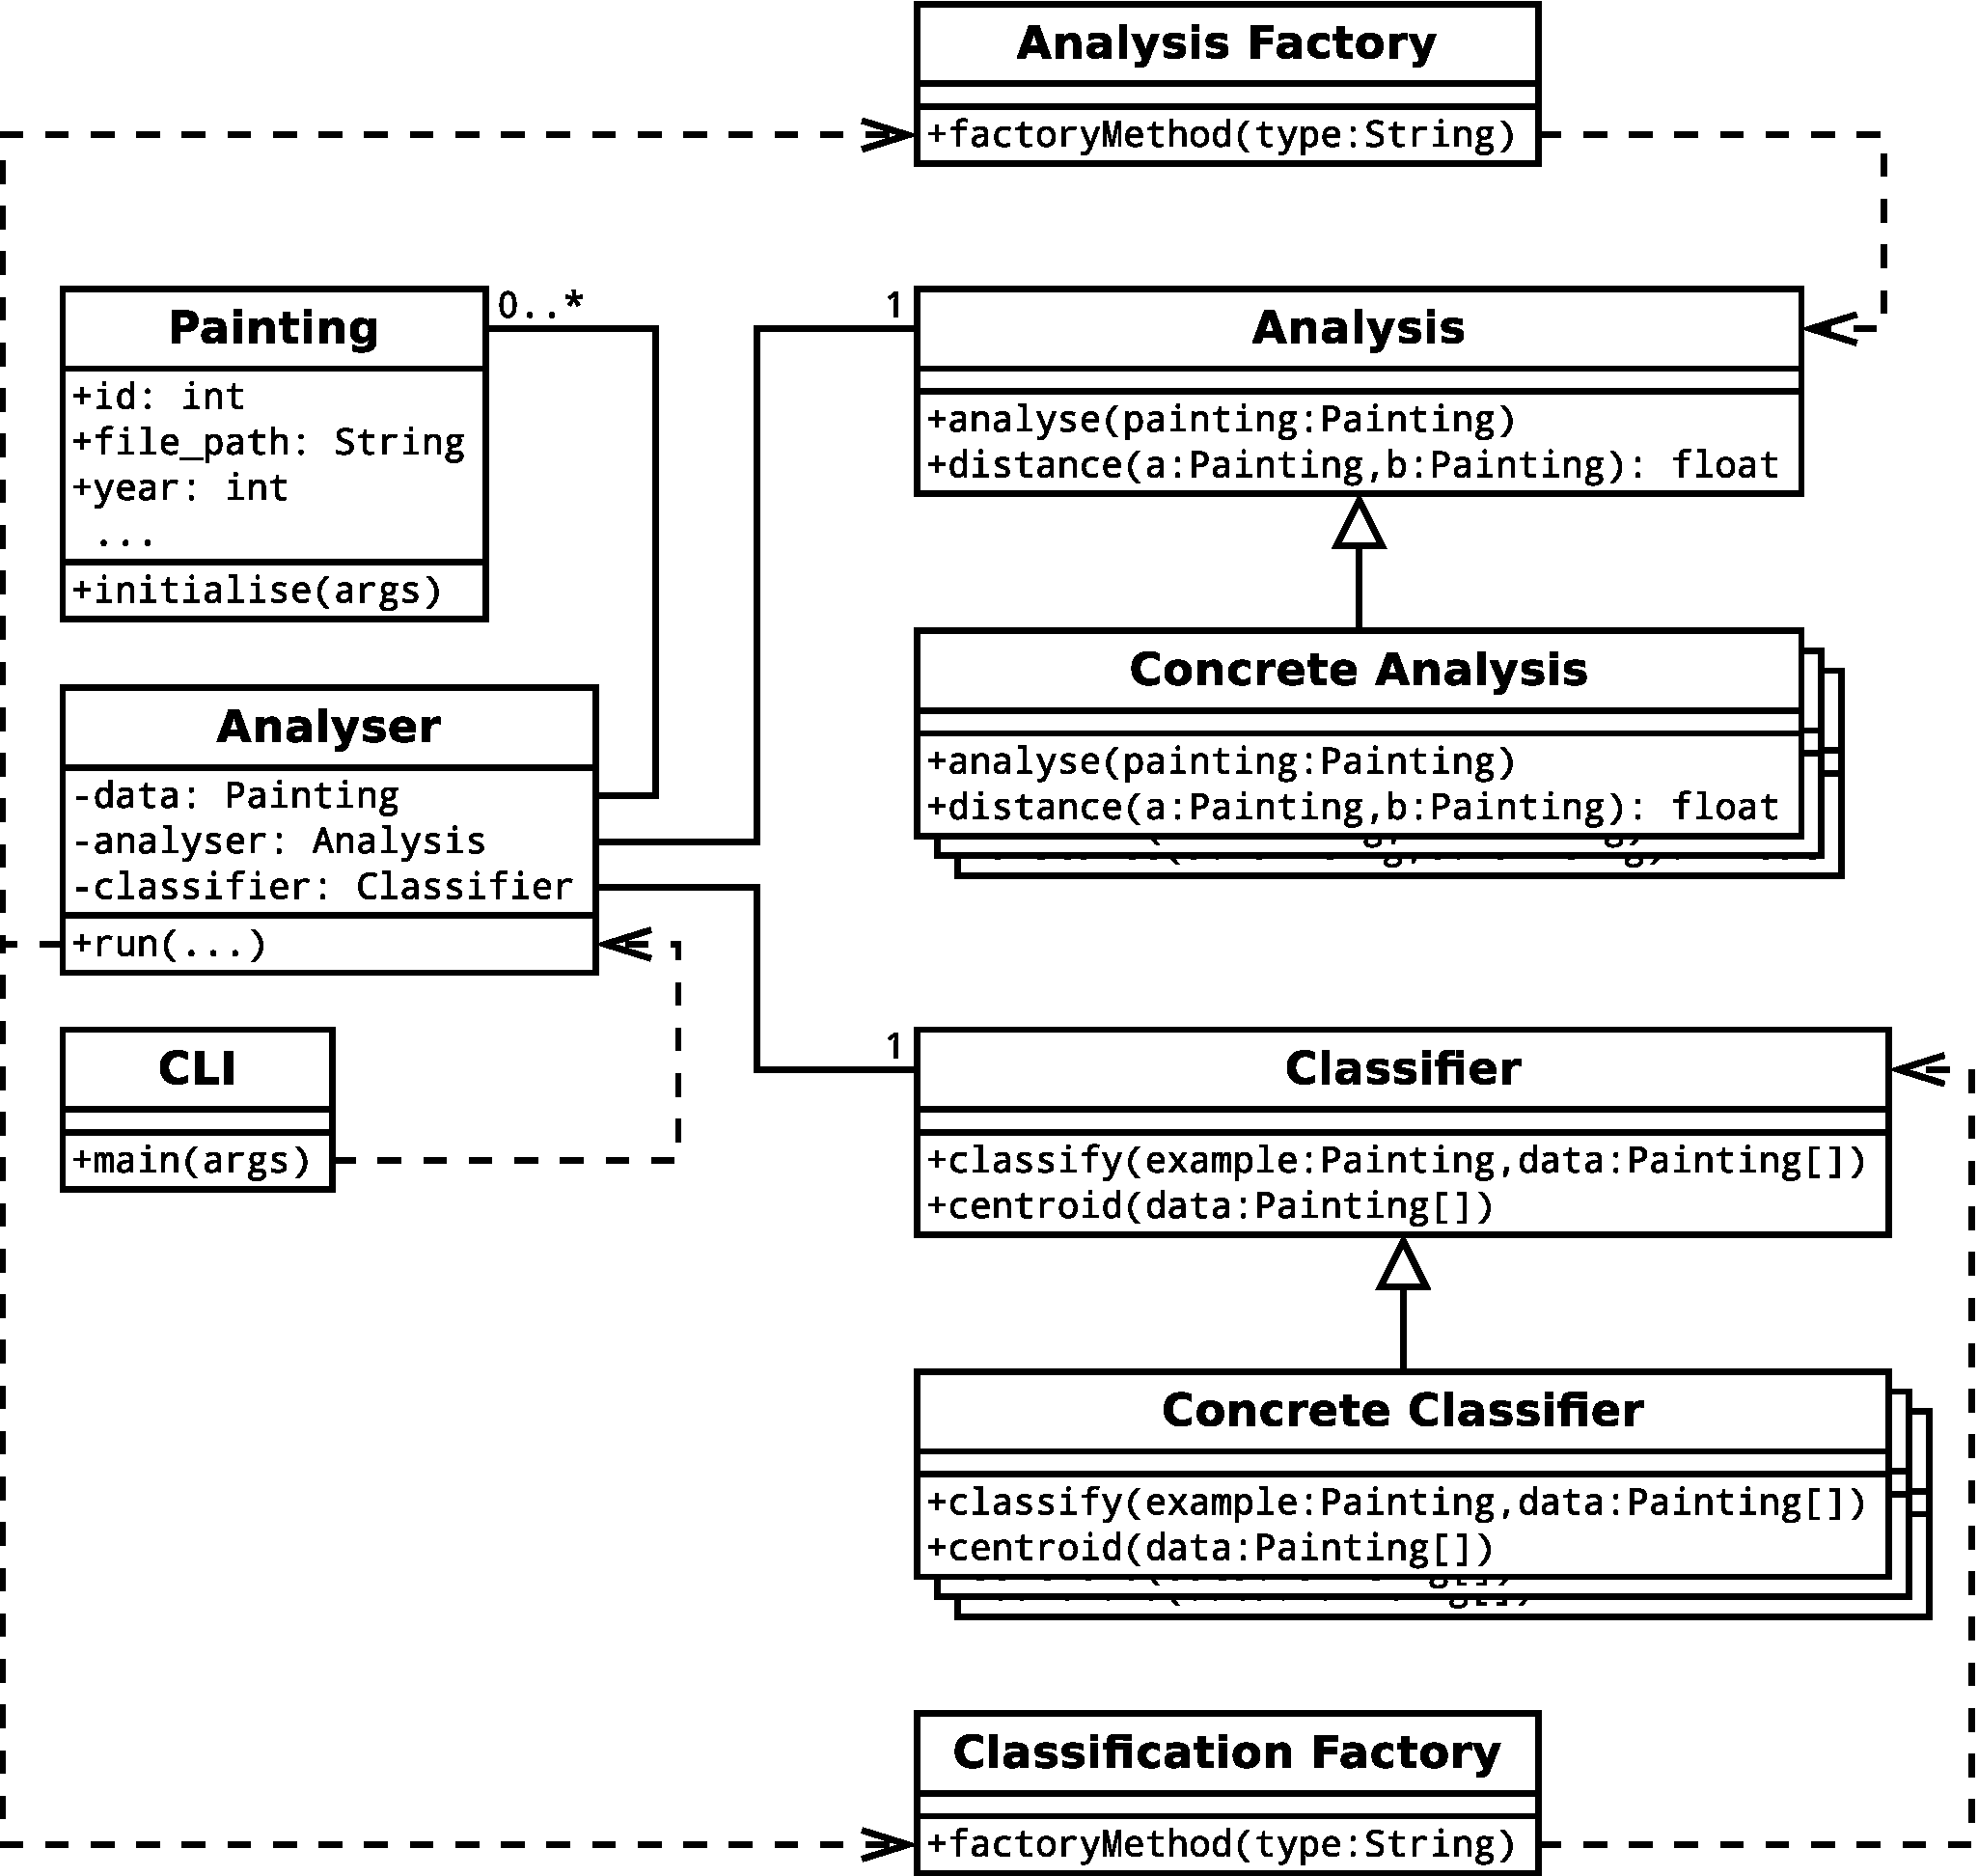
\includegraphics[width=\textwidth]{img/uml-final}
\caption{Final class design}\label{fig:uml-final}
\end{figure}
